
\section{Search-R1}

\begin{figure}
    \centering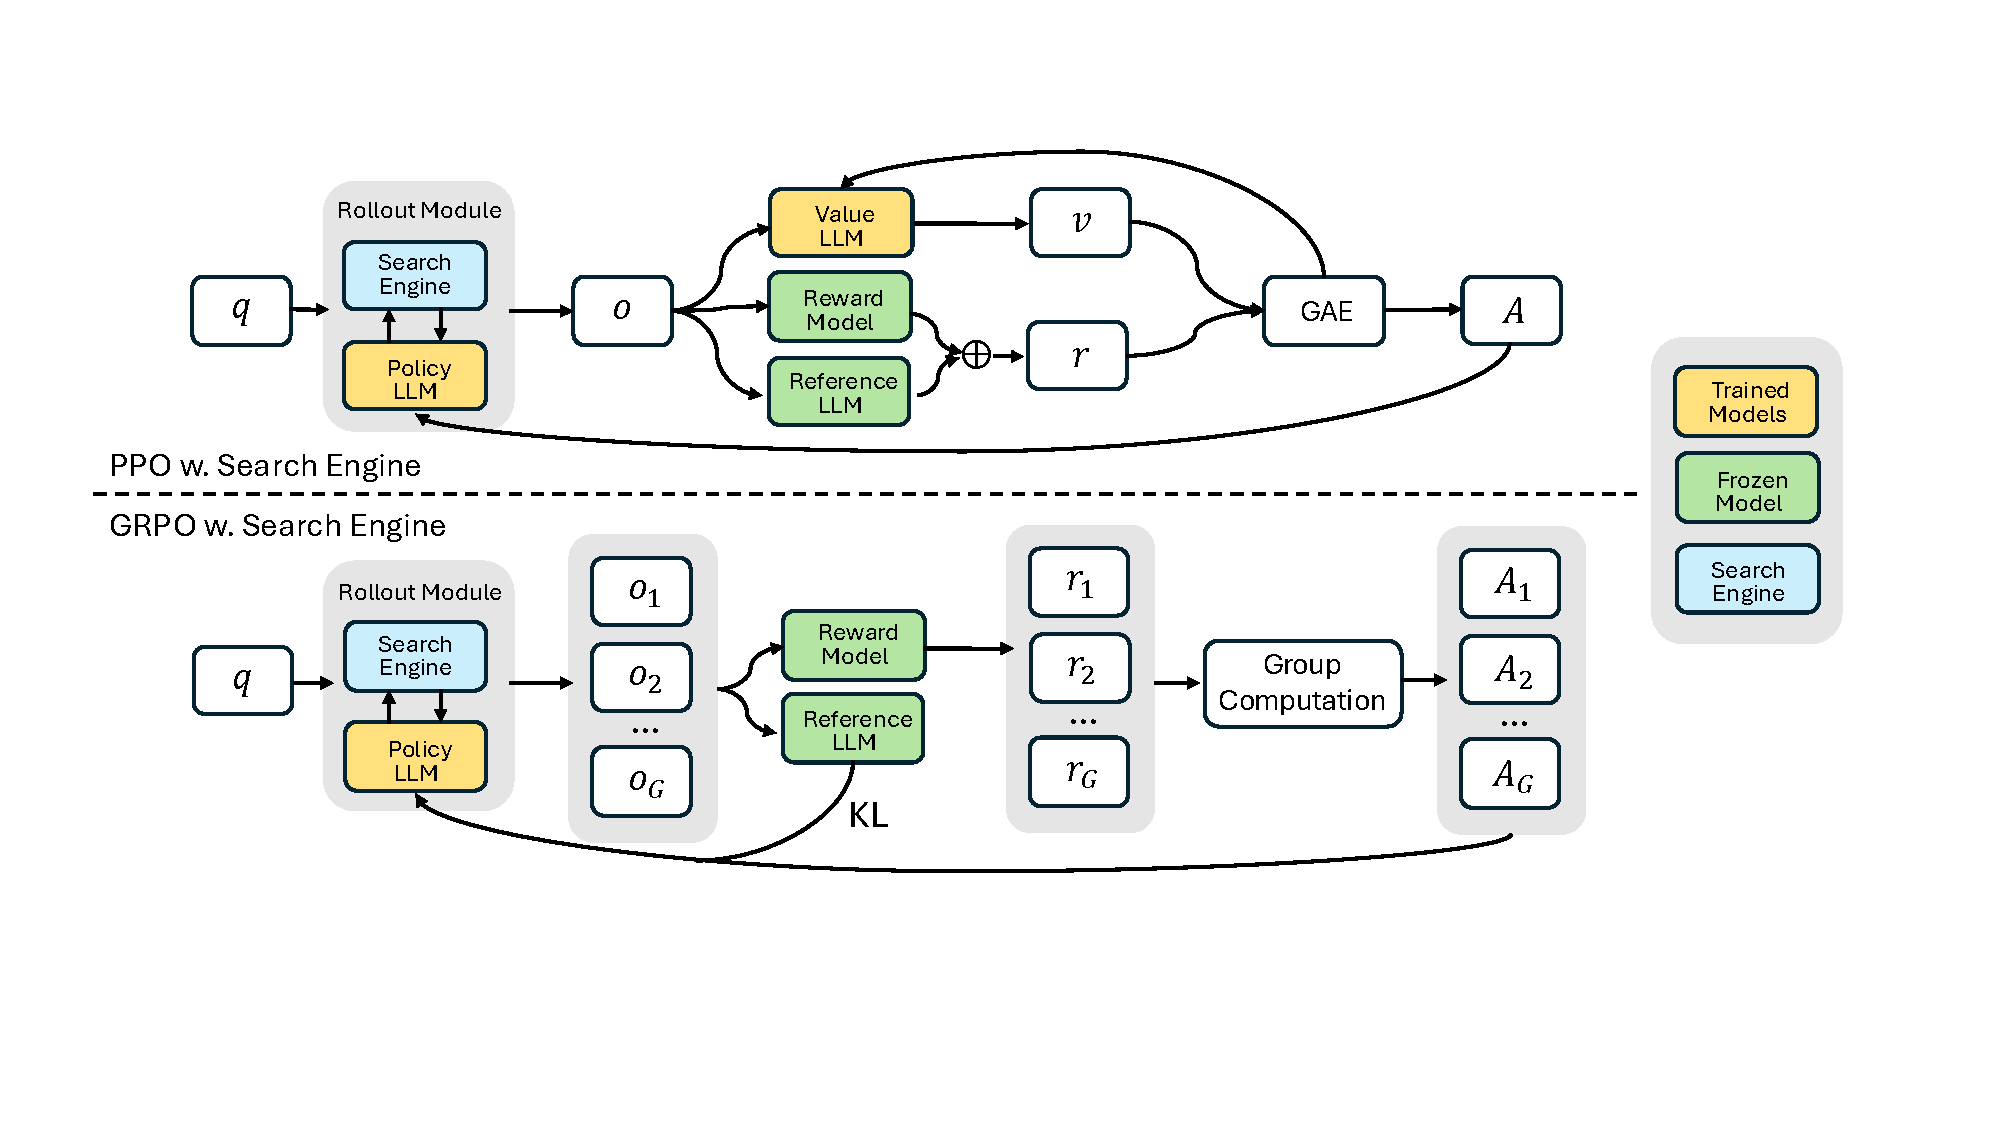
\includegraphics[width=1.0\textwidth,trim="0 0 0 .2cm",clip]{figures/main.pdf}
    \caption{Demonstration of PPO and GRPO training with the search engine (\Ours). During the rollout, LLMs can conduct multi-turn interactions with the search engine.}\label{fig:main}
\end{figure}

In the following sections, we present the detailed design for training methods of \Ours, covering (1) extending RL to utilize search engines; (2) text generation with an interleaved multi-turn search engine call; (3) the training template; and (4) reward model design.

\subsection{Reinforcement Learning with a Search Engine}

% The reinforcement learning framework with a search engine $\text{Ret}(\cdot)$ can be formulated as follows:
We formulate the RL objective function utilizing a search engine $\se$ as follows:
% {\scriptsize
\begin{gather}\label{eq:rl-retriever}
    \max_{\pi_\theta} \mathbb{E}_{x \sim \mathcal{D}, y \sim \pi_{\theta}(\cdot \mid x; \se)} 
\left[ r_{\phi}(x, y) \right] 
- \beta \mathbb{D}_{\text{KL}} \left[ \pi_{\theta}(y \mid x; \se) \,||\, \pi_{\text{ref}}(y \mid x; \se) \right],
\end{gather}
% }
where $\pi_{\theta}$ is the policy LLM, $\pi_{\text{ref}}$ is the reference LLM, $r_{\phi}$ is the reward function and $\mathbb{D}_{\text{KL}}$ is KL-divergence measure.
\( x \) denote input samples drawn from the dataset \( \mathcal{D} \), and \( y \) represent the generated outputs interleaved with search engine calling results, sampled from the reference policy \( \pi_{\text{ref}}(y \mid x) \) and retrieved from the search engine $\se$. 
Unlike prior RL approaches that primarily rely on the policy LLM $\pi_{\theta}(\cdot \mid x)$ to generate rollout sequences \citep{rafailov2023direct, ouyang2022training}, our framework explicitly incorporates retrieval interleaved reasoning via $\pi_{\theta}(\cdot \mid x; \se)$, which can be seen as $\pi_{\theta}(\cdot \mid x) \bigotimes \se$, where $\bigotimes$ denotes interleaved retrieval-and-reasoning.
This enables more effective decision-making in reasoning-intensive tasks that require external information retrieval. An illustration of the rollout process and an explanation of Eq. \ref{eq:rl-retriever} are provided in Section \ref{sec:rollout} and Appendix \ref{sec:apx:rl-formulation}.

% \hamed{$\pi_{ref}$ is not defined here. $D_{KL}$ is not defined either, even though it's obvious, everything should be defined.} 
% \hamed{you don't have max in the next two equation, so better to be consistent here as well and drop max and define this as an objective function.}

% Different from previous LLM reinforcement learning method that mainly rely on policy LLM $\pi_{\theta}(\cdot \mid x)$ to generate the rollout sequence \citep{rafailov2023direct, ouyang2022training}, in our reasoning + search scenarios, the rollout sequence $y$ for a prompt is generated by interleaved reasoning $\pi_{\theta}(\cdot \mid x)$ and search engine calling $\text{Ret}(\cdot)$.
% The detailed illustration can be found in Section \ref{sec:rollout}.

Our approach builds upon two well-established policy gradient RL methods: Proximal Policy Optimization (PPO) \citep{schulman2017proximal} and Group Relative Policy Optimization (GRPO) \citep{shao2024deepseekmath,guo2025deepseek}, leveraging their respective advantages to optimize retrieval-augmented reasoning.

\paragraph{Loss Masking for Retrieved Tokens.}\label{sec:kl-mask}

In both PPO and GRPO, the token-level losses are computed over the entire rollout sequence. In \Ours, the rollout sequence consists of both LLM-generated tokens and retrieved tokens from external passages.
While optimizing LLM-generated tokens enhances the model’s ability to interact with the search engine and perform reasoning, applying the same optimization to retrieved tokens can lead to unintended learning dynamics. To address this, we introduce loss masking for retrieved tokens, ensuring the policy gradient objective is computed only over LLM-generated tokens, excluding retrieved content from the optimization process. This approach stabilizes training while preserving the flexibility of search-augmented generation.

\paragraph{PPO with Search Engine.}

Proximal Policy Optimization (PPO) \citep{schulman2017proximal} is a popular actor-critic RL approach commonly used for LLMs \citep{ouyang2022training}.
For our reasoning scenarios that involve search engine calling, it optimizes LLMs by maximizing the following objective:
{\scriptsize
\begin{gather}\label{eq:ppo}
\mathcal{J}_{PPO}(\theta) = \mathbb{E}_{x \sim \mathcal{D}, y \sim \pi_{\text{old}}( \cdot| x; \se)}
\left[ \frac{1}{\sum_{t=1}^{|y|} I(y_t)} \sum_{t=1: I(y_t)=1}^{|y|}
\min \left( \frac{\pi_{\theta}(y_t | x, y_{<t}; \se)}{\pi_{\text{old}}(y_t | x, y_{<t}; \se)} A_t, 
\text{clip} \left( \frac{\pi_{\theta}(y_t | x, y_{<t}; \se)}{\pi_{\text{old}}(y_t | x, y_{<t}; \se)}, 1 - \epsilon, 1 + \epsilon \right) A_t 
\right) \right],
\end{gather}}
where \( \pi_{\theta} \) and \( \pi_{\text{old}} \) represent the current and previous policy models, respectively. 
% \( x \) denote input samples drawn from the dataset \( \mathcal{D} \), and \( y \) represent the generated outputs interleaved with search engine calling results, sampled from the reference policy \( \pi_{\text{ref}}(y \mid x; \se) \) and retrieved from the search engine $\se$. 
$I(y_t)$ is the token loss masking operation such that $I(y_t)=1$ if $y_t$ is a LLM generated token and $I(y_t)=0$ if $y_t$ is a retrieved token.
The term \( \epsilon \) is a clipping-related hyperparameter introduced in PPO to stabilize training. 
The advantage estimate \( A_t \) is computed using Generalized Advantage Estimation (GAE) \citep{schulman2015high}, based on future rewards \( \{ r_{\geq t} \} \) and a learned value function \( V_{\phi} \).


\paragraph{GRPO with Search Engine.}

To improve policy optimization stability and avoid the need for an additional value function approximation, Group Relative Policy Optimization (GRPO) is introduced in \cite{shao2024deepseekmath}. GRPO differs from PPO by leveraging the average reward of multiple sampled outputs as a baseline rather than relying on a learned value function. Specifically, for each input question \( x \), GRPO samples a group of responses \( \{ y_1, y_2, \dots, y_G \} \) from the reference policy \( \pi_{\text{ref}} \). The policy model is then optimized by maximizing the following objective function:
{\scriptsize
\begin{align}\label{eq:grpo}
\mathcal{J}_{GRPO}(\theta) = \, & 
\mathbb{E}_{x \sim \mathcal{D}, \{ y_i \}_{i=1}^{G} \sim \pi_{\text{old}}( \cdot| x; \se)}
\Bigg[
\frac{1}{G} \sum_{i=1}^{G} \frac{1}{\sum_{t=1}^{|y_i|}  I(y_{i,t})} \sum_{t=1: I(y_{i,t})=1}^{|y_i|} 
\min \Bigg( 
\frac{\pi_{\theta}(y_{i,t} | x, y_{i,<t}; \se)}{\pi_{\text{old}}(y_{i,t} | x, y_{i,<t}; \se)} \hat{A}_{i,t}, 
\nonumber \\[8pt] 
& \hspace{120pt} \text{clip} \Bigg( \frac{\pi_{\theta}(y_{i,t} | x, y_{i,<t}; \se)}{\pi_{\text{old}}(y_{i,t} | x, y_{i,<t}; \se)}, 1 - \epsilon, 1 + \epsilon \Bigg) \hat{A}_{i,t} 
\Bigg)
- \beta \mathbb{D}_{KL} \left[ \pi_{\theta} || \pi_{\text{ref}} \right]
\Bigg],
\end{align}
}
where \( \epsilon \) and \( \beta \) are hyperparameters, and \( \hat{A}_{i,t} \) represent the advantage, computed based on the relative rewards of outputs within each group. 
This approach avoids introducing additional complexity in the computation of \( \hat{A}_{i,t} \).
% $I(y_{i,t})$ is the token loss masking operation. $I(y_{i,t})=1$ if $y_{i,t}$ are LLM generated tokens and $I(y_{i,t})=0$ if $y_{i,t}$ are retrieved tokens.
Additionally, instead of incorporating KL divergence as a penalty within the reward function, GRPO regularizes by directly adding the KL divergence between the trained policy and the reference policy to the loss function. 
The retrieved token masking is also applied when calculating the KL divergence loss $\mathbb{D}_{KL}$.


\subsection{Generation with Multi-turn Search Engine Calling}\label{sec:rollout}

In this section, we describe the rollout process for LLM response generation with interleaved multi-turn search engine calls, formulated as: $y\sim \pi_{\theta}(\cdot \mid x; \se) = \pi_{\theta}(\cdot \mid x) \bigotimes \se$.

Our approach follows an iterative framework where the LLM alternates between text generation and external search engine queries. Specifically, the system instruction guides the LLM to encapsulate its search query between two designated search call tokens, \search{and}, whenever an external retrieval is needed. Upon detecting these tokens in the generated sequence, the system extracts the search query, queries the search engine, and retrieves relevant results.
The retrieved information is then enclosed within special retrieval tokens, \info{and}, and appended to the ongoing rollout sequence, serving as additional context for the next generation step. 
This process continues iteratively until one of the following conditions is met: (1) the maximum number of action is reached, or (2) the model generates a final response, which is enclosed between designated answer tokens, \answer{and}.
The complete workflow is outlined in Algorithm \ref{alg:llm_search}.


\begin{algorithm}[t]
\caption{LLM Response Rollout with Multi-Turn Search Engine Calls}
\label{alg:llm_search}
\begin{algorithmic}[1]
\Require Input query \( x \), policy model \( \pi_{\theta} \), search engine \( \se \), maximum action budget \( B \).
\Ensure Final response \( y \).

\State Initialize rollout sequence \( y \gets \emptyset \)
% \State Initialize search call count \( b \gets 0 \)
\State Initialize action count \( b \gets 0 \)

\While{\( b < B \)}
    \State Initialize current action LLM rollout sequence \( y_b \gets \emptyset \) 
    \While{True}
    \State Generate response token \( y_t \sim \pi_{\theta}(\cdot \mid x, y + y_b) \)
    \State Append \( y_t \) to rollout sequence \( y_b \gets y_b + y_t \)
    \If{\( y_t \) in [\textcolor{cyan}{\texttt{</search>}}, \textcolor{purple}{\texttt{</answer>}}, \texttt{<eos>}]}
        break
    \EndIf
    \EndWhile

    \State \( y  \gets  y + y_b \)
    \If{\search{} detected in \( y_b \)}
        \State Extract search query \( q \gets \text{Parse}(y_b, \search{,} ) \)
        \State Retrieve search results \( d = \se(q) \)
        \State Insert $d$ into rollout \( y  \gets  y + \info{d}  \)
    \ElsIf{\answer{} detected in \( y_b \)}
        % \State // \textcolor{cvprblue}{Terminate rollout}
        \State \textbf{return} final generated response \( y \)
    \Else
        \State Ask for rethink \( y  \gets  y + \) ``My action is not correct. Let me rethink.''
    \EndIf

    \State Increment action count \( b \gets b + 1 \)
\EndWhile

\State \textbf{return} final generated response \( y \)
\end{algorithmic}
\end{algorithm}


\subsection{Training Template}

To train \Ours, we start by crafting a simple template that directs the initial LLM to follow our predefined instructions. 
As shown in Table \ref{tab:instruction}, this template structures the model’s output into three parts in an iterative fashion: first, a reasoning process, then a search engine calling function, and finally, the answer. 
We deliberately limit our constraints to this structural format, avoiding any content-specific biases, such as enforcing reflective reasoning and search engine calling or endorsing specific problem-solving approaches. 
This ensures that the model’s natural learning dynamics during the RL process remain observable and unbiased.


\begin{table}[h]
    \centering
    \begin{tabular}{p{13cm}}
        \hline
        Answer the given question. \
        You must conduct reasoning inside \think{and} first every time you get new information. \
        After reasoning, if you find you lack some knowledge, you can call a search engine by \search{query}, and it will return the top searched results between \info{and}. \
        You can search as many times as you want. \
        If you find no further external knowledge needed, you can directly provide the answer inside \answer{and} without detailed illustrations. For example, \answer{xxx}. Question: \textcolor{red}{question}.\\
        \hline
    \end{tabular}
    \caption{Template for \Ours. \textcolor{red}{question} will be replaced with the specific question during training and inference.}\label{tab:instruction}
\end{table}


\subsection{Reward Modeling}

The reward function serves as the primary training signal, guiding the optimization process in RL. To train \Ours, we adopt a rule-based reward system that consists solely of \textbf{final outcome rewards}, which assess the correctness of the model’s response. For instance, in factual reasoning tasks, correctness can be evaluated using rule-based criteria such as exact string matching:
\begin{gather}
    r_{\phi}(x, y) = \text{EM}(a_\text{pred}, a_\text{gold}),
\end{gather}
where $a_\text{pred}$ is the extracted final answer from response $y$ and $a_\text{gold}$ is the ground truth answer.
% \hamed{please leave an equation somewhere that defined the exact formulation of $A_t$ function. This textual description can be a bit ambiguous.}
Unlike \cite{guo2025deepseek}, we do not incorporate format rewards, as our learned model already demonstrates strong structural adherence. We leave the exploration of more complex format rewards for future work. Furthermore, we avoid training neural reward models, following \cite{guo2025deepseek}. This decision is motivated by the sensitivity of LLMs to specific forms of rewards in large-scale RL, as well as the additional computational cost and complexity introduced by retraining these models.
